\section{Heapsort}

\subsection{Heaps}

\begin{description}
  \descitem{6.1-1} \textit{What are the minimum and maximum numbers of elements in a heap of height $h$?} %TODO:TikZ heap diagram
    \begin{ex}
      \begin{itemize}
        \item Minimum : $2^{h}$ ;
        \item Maximum : $2^{h+1}-1$.
      \end{itemize}
    \end{ex} 
  \descitem{6.1-2} \textit{Show that an $n$-element heap has height $\lfloor \lg n \rfloor$.}
    \begin{ex}
      On reprend le r\'esultat pr\'ec\'edent (exercice \descref{6.1-1})  qui nous offre l'in\'egalit\'e :
      \[2^h \le n \le 2^{h+1}-1.\]
      Ainsi, \'etant donn\'e un nombre d'\'el\'ements $n$, l'hauteur $h$ d'un tas est born\'ee par :
      \[\lg n -1  < \lg(n+1)-1 \le h \le \lg n.\]
      Sachant que $h$ est un entier, \`a partir de $\lg n - 1 < h \le \lg n$ on d\'eduit que $h = \lfloor \lg n \rfloor$.
    \end{ex}
  \descitem{6.1-3} \textit{Show that in any subtree of a max-heap, the root of the subtree contains the largest value occurring anywhere in that subtree.}
    \begin{ex} %TODO:give a complet proove
      C'est une cons\'equence imm\'ediate de la propri\'et\'e d'un \textit{max-heap} : la cl\'e de la racine d'un sous-arbre est sup\'erieur \'egale \`a celle de ses enfants; or, ses enfants sont \'egalement la racine du sous-arbre qu'ils apartiennent. De ce fait, une preuve plus compl\`ete serait achev\'ee par induction math\'ematiques.
    \end{ex}
  \descitem{6.1-4} \textit{Where in a max-heap might the smallest element reside, assuming that all elements are distinct?}
    \begin{ex}
      La propri\'et\'e d'un \textit{max-heap} est que $A[\proc{Parent}(i)] \ge A[i]$ ce qui signifit que tout chemin partant de la racine forme une suite d\'ecroissante, et strictement, par hypoth\`ese. Par cons\'equence, le plus petit \'el\'ement r\'eside dans une des feuilles. Ce r\'esultat d\'ecoule du fait que la relation d'ordre n'est pas totale sur le tas.
    \end{ex}
  \descitem{6.1-5} \textit{Is an array that is in sorted order a min-heap?}
    \begin{ex} %TODO:add proof
      Si le tableau est tri\'e de mani\`ere croissante, le tableau forme un \textit{min-heap}.
    \end{ex}
  \descitem{6.1-6} \textit{Is the array with values $\langle 23, 17, 14, 6, 13, 10, 1, 5, 7, 12\rangle$ a max-heap?}
    \begin{ex}
      Consid\'erons la figure (\ref{fig:6.1-6}) qui est la repr\'esentation arborescente du tableau. On voit qu'il existe une sous-suite qui n'est pas d\'ecroissante : $(23, 17, 6, 7)$, donc ce tableau ne v\'erifie pas la propri\'et\'e d'un \textit{max-heap}.
        \begin{figure}[t]
          \centering
        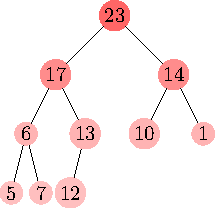
\includegraphics[scale=1.5]{img/6_1-6/6_1-6.pdf}
        \caption{Tas sous forme d'arbre du tableau $\langle 23, 17, 14, 6, 13, 10, 1, 5, 7, 12\rangle$}
          \label{fig:6.1-6}
        \end{figure}
    \end{ex}
  \descitem{6.1-7} \textit{Show that, with the array representation for storing an $n$-element heap, the leaves are the nodes indexed by $\lfloor n/2 \rfloor +1, \lfloor n/2\rfloor + 2, \ldots, n$.}
    \begin{ex}
      Une feuille n'a pas de fils, et comme les n\oe ux sont ins\'er\'es de fa\c{c}on contig\"ue, il suffit de trouver le premier    $k$ tel que $\textsc{Left}(k) =2k > n$. On a donc $n/2 < k$ et puis comme $k$ est un entier, il vaut $\lfloor n/2 \rfloor +1$.
    \end{ex}
\end{description}

\subsection{Maintaining the heap property}

\begin{description}
  \descitem{6.2-1} \textit{Using Figure 6.2 as a model, illustrate the operation of $\proc{Max-Heapify}(A,3)$ on the array $A = \langle 27, 17, 3, 16, 13, 10, 1, 5, 7, 12, 4, 8, 9, 0 \rangle$}
    \begin{ex}

      Regardons la figure (\ref{fig:Heapify}) qui illustre les op\'erations de $\proc{Max-Heapify}(A,3)$ : (\subref{fig:6_2-1_1}) La configuration initiale du tas, avec la valeur $A[3]$ au n\oe ud $i = 3$ viole la propri\'et\'e de \textit{max-heap} puisque'elle n'est pas sup\'erieur \`a celle des enfants. La propri\'et\'e de \textit{max-heap} est restaur\'ee pour le n\oe ud $3$ en (\subref{fig:6_2-1_2}) via \'echange de $A[3]$ avec $A[6]$, ce qui d\'etruit la propri\'et\'e de \textit{max-heap} pour le n\oe ud $6$. L'appel r\'ecursif $\proc{Max-Heapify}(A,6)$ prend maintenant $i=6$. Apr\`es  avoir \'echang\'e $A[6]$ avec $A[13]$, comme illustr\'e en (\subref{fig:6_2-1_3}), le n\oe ud $6$ est corrig\'e, et l'appel r\'ecursif $\proc{Max-Heapify}(A,13)$ n'engendre plus de modifications de la structure de donn\'ees.

      \begin{figure}[t]
        \centering
        \begin{subfigure}[t]{.45\textwidth}
          \centering
          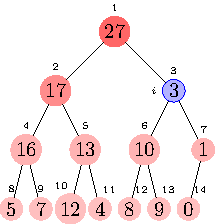
\includegraphics[scale=1.4]{img/6_2-1/6_2-1_1}
          \caption{}\label{fig:6_2-1_1}
        \end{subfigure}

        \begin{subfigure}[t]{.45\textwidth}
          \centering
          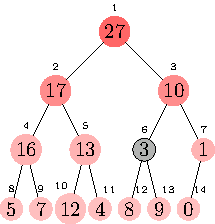
\includegraphics[scale=1.4]{img/6_2-1/6_2-1_2}
          \caption{}\label{fig:6_2-1_2}
        \end{subfigure}
        \begin{subfigure}[t]{.45\textwidth}
          \centering
          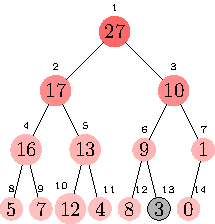
\includegraphics[scale=1.4]{img/6_2-1/6_2-1_3}
          \caption{}\label{fig:6_2-1_3}
        \end{subfigure}
        \caption{L'action $\proc{Max-Heapify}(A,3)$,o\`u $\attrib{A}{heap-size}= 14$.} 
        \label{fig:Heapify}
      \end{figure}
    \end{ex}
  \descitem{6.2-2} \textit{Starting with the procedure \proc{Max-Heapify}, write pseudocode for the procedure $\proc{Min-Heapify}(A,i)$ which performs the corresponding manipulation on a min-heap. How does the running time of \proc{Min-Heapify} compare to that of \proc{Max-Heapify} ?}
    \begin{ex}
      \begin{codebox}
        \Procname{\algo{Min-Heapify}$(A,i)$}
        \li $l = \proc{Left}(i)$
        \li $r = \proc{Right}(i)$
        \li \If $l \le \attrib{A}{heap-size}$ and $A[l] < A[i]$ \Do
        \li $\id{least} = l$        
        \li \Else $\id{least} = i$ \End
        \li \If $r \le \attrib{A}{heap-size}$ and $A[r] < A[least]$ \Do
        \li $\id{least} = r$  \End    
        \li \If $\id{least} \ne i$ \Do
        \li $\func{swap}(A,i,\id{least})$
        \li $\proc{Min-Heapify}(A,least)$
      \end{codebox}
      L'algorithme \'etant la m\^eme que celle du \proc{Max-Heapify} \`a quelques signes pr\`es, on est certain qu'ils ont la m\^eme complexit\'e en temps. D\'etaillons quand m\^eme la preuve du livre. 
      Le temps d'ex\'ecution de \proc{Min-Heapify} est le temps $\Theta(1)$ n\'ecessaire pour corriger les relations entre les \'el\'ements, plus le temps d'ex\'ecuter \proc{Min-Heapify} sur un sous-arbre enracin\'e sur l'un des enfants du n\oe ud $i$. 
      
      Majorons la taille du sous-arbre de gauche.  On sait que le pire des cas survient quand la derni\`ere rang\'ee de l'arbre est remplie \`a moiti\'e, alors on a la ratio suivant : 
      \[R_n = \frac{\textrm{taille de l'arbre enracin\'e sur le n\oe ud  } \proc{Left}(i)}{\textrm{taille de l'arbre enracin\'e sur le n\oe ud } i} = \frac{2^{n-1}-1}{2^n-2^{n-2}-1}.\]
      $R_n$ est croissante et admet une limite $R_n \underset{n \to +\infty}{\longrightarrow} 2/3$ qui est le major\'e de la taille du sous-arbre de gauche. Ainsi, on obtient l'in\'egalit\'e : \[T(n) \le T(2n/3) + \Theta(1).\]
      Puis on utilise le \textit{master theorem}. Dans notre cas $f(n) = \Theta(1)$ et $n^{\log_{3/2}1} = 1$. Le deuxi\`eme cas convient, on a bien $f(n) = \Theta(1)$, donc la solution est $T(n) = O(\lg n) = O(h)$ avec $h$ l'hauteur de l'arbre (d'apr\`es \descref{6.1-2}, $h = \lfloor \lg n \rfloor$). 
    \end{ex}
  \descitem{6.2-3} \textit{What is the effect of calling $\proc{Max-Heapify}(A,i)$ when the element $A[i]$ is larger than its children?}
    \begin{ex}
      L'algorithme effectue les comparaisons n\'ecessaires et s'arr\^ete en temps constant. Aucun \'echange a lieu car le n\oe ud et ses fils v\'erifient la propri\'et\'e d'un \textit{max-heap}.
    \end{ex}
  \descitem{6.2-4} \textit{What is the effect of calling $\proc{Max-Heapify}(A,i)$ for $i > \attrib{A}{heap-size}/2$?}
    \begin{ex}
      On a $\lfloor \attrib{A}{heap-size}/2 \rfloor + 1 \le i \le \attrib{A}{heap-size}$, d'apr\`es \descref{6.1-7}, tous les n\oe ud d'indice $i$ sont des feuilles. Donc l'algorithme s'arr\^ete en temps constant et aucun \'echange a lieu.
    \end{ex}
  \descitem{6.2-5} \textit{The code for \proc{Max-Heapify} is quite efficient in terms of constant factors, except
possibly for the recursive call in line 10, which might cause some compilers to
produce inefficient code. Write an efficient \proc{Max-Heapify} that uses an iterative
control construct (a loop) instead of recursion.}
    \begin{ex}
      \begin{codebox}
        \Procname{\algo{Iterative-Max-Heapify}$(A,i)$}
        \li \While $\proc{Left}(i) < \attrib{A}{heap-size}$ and $\proc{Right}(i) < \attrib{A}{heap-size}$ \Do
        \li $l = \proc{Left}(i)$
        \li $r = \proc{Right}(i)$
        \li \Comment Les lignes \ref{li:IMH-begin-compare}-\ref{li:IMH-end-compare} peuvent \^etre exprimer autrement
      \footnote{$\id{largest} = \func{index-of-max}(A[i], A[l], A[r])$.}
        \li \If  $A[l] > A[i]$ \Do           \label{li:IMH-begin-compare} 
        \li $\id{largest} = l$        
        \li \Else $\id{largest} = i$ \End
        \li \If  $A[r] > A[largest]$ \Do
        \li $\id{largest} = r$  \End         \label{li:IMH-end-compare}
        \li \If $\id{largest} \ne i$ \Do
        \li $\func{swap}(A,i,\id{largest})$ 
        \li $i = \id{largest}$
        \li \Else \Return \End
        \End 
      \end{codebox}
    \end{ex}
  \descitem{6.2-6} \textit{Show that the worst-case running time of \proc{Max-Heapify} on a heap of size $n$
is $\Omega(\lg n)$. (Hint: For a heap with $n$ nodes, give node values that cause \proc{Max-Heapify}
 to be called recursively at every node on a simple path from the root down to a leaf.)}
    \begin{ex}
      Le pire cas a lieu lorsqu'il existe un chemin tel que ses \'el\'ements sont tri\'es de mani\`ere croissante. Dans ce cas l\`a, il y a exactement $h = \lfloor \lg n\rfloor$ appels recursives de la fonction \proc{Max-Heapify}. D'o\`u la borne inf\'erieure $\Omega(\lg n)$.
    \end{ex} 
\end{description}

\subsection{Building a heap}

\begin{description}
    \descitem{6.3-1} \textit{Using Figure 6.3 as a model, illustrate the operation of \proc{Build-Max-Heap} on the
array $A = \langle 5, 3, 17, 10, 84, 19, 6, 22, 9 \rangle$.}
    \begin{ex}
	 Observons la figure (\ref{fig:Build-Max-Heap}) : (\subref{fig:6_3-1_1}) Un tableau de 9 \'el\'ements en entr\'ee, avec l'arbre binaire qu'il repr\'esente. La figure montre que l'indice de boucle $i$ pointe vers le n\oe ud 4 avant l'appel $\proc{Max-Heapify}(A,i)$. (\subref{fig:6_3-1_2}) La structure de donn\'ees r\'esultante. L'indicde de boucle $i$ de l'it\'eration suivante pointe vers le n\oe ud $3$. (\subref{fig:6_3-1_3})-(\subref{fig:6_3-1_4}) Les it\'erations suivantes de la boucle \textbf{for} de \proc{Build-Max-Heap}. \`A chaque fois qu'il y a appel de \proc{Max-Heapify} sur un n\oe ud, les deux sous-arbres de ce n\oe ud sont des \textit{max-heap}. (\subref{fig:6_3-1_5}) Le \textit{max-heap} apr\`es que \proc{Build-Max-Heap} a fini.
      \begin{figure}[H]
        \centering
        \begin{subfigure}[t]{.45\textwidth}
          \centering
          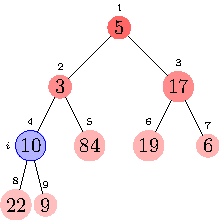
\includegraphics[scale=1.4]{img/6_3-1/6_3-1_1}
          \caption{}\label{fig:6_3-1_1}
        \end{subfigure}
        \begin{subfigure}[t]{.45\textwidth}
          \centering
          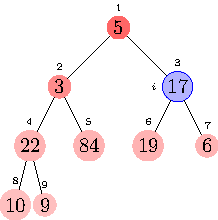
\includegraphics[scale=1.4]{img/6_3-1/6_3-1_2}
          \caption{}\label{fig:6_3-1_2}
        \end{subfigure}
        \begin{subfigure}[t]{.45\textwidth}
          \centering
          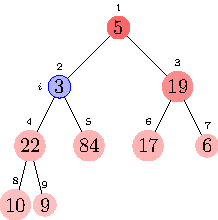
\includegraphics[scale=1.4]{img/6_3-1/6_3-1_3}
          \caption{}\label{fig:6_3-1_3}
        \end{subfigure}
        \begin{subfigure}[t]{.45\textwidth}
          \centering
          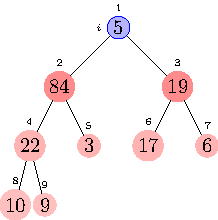
\includegraphics[scale=1.4]{img/6_3-1/6_3-1_4}
          \caption{}\label{fig:6_3-1_4}
        \end{subfigure}
        \begin{subfigure}[t]{.45\textwidth}
          \centering
          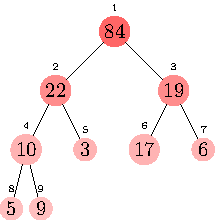
\includegraphics[scale=1.4]{img/6_3-1/6_3-1_5}
          \caption{}\label{fig:6_3-1_5}
        \end{subfigure}
        \caption{Le fonctionnement de $\proc{Build-Max-Heap}(A)$, o\`u $\attrib{A}{heap-size}= 9$.} 
        \label{fig:Build-Max-Heap}
      \end{figure}
    \end{ex}
    \descitem{6.3-2} \textit{Why do we want the loop index $i$ in line 2 of \proc{Build-Max-Heap} to decrease from
$\lfloor \attrib{A}{length}/2 \rfloor$ to $1$ rather than increase from $1$ to $\lfloor \attrib{A}{length}/2 \rfloor$ ?}
    \begin{ex}
	  L'hypoth\`ese de $\proc{Max-Heapify}(A,i)$ est que les sous-arbres $\proc{Left}(i)$ et $\proc{Right}(i)$ sont des \textit{max-heap}s. Si l'on commence par le n\oe ud $1$, alors il n'y a aucune garantie que les n\oe uds parcourus seront toujours des \textit{max-heap}s.
    \end{ex}
    \descitem{6.3-3} \textit{Show that there are at most $\lceil n/2^{h+1}\rceil$ nodes of height $h$ in any $n$-element heap.}
    \begin{ex} %TODO:relire et changer les notations
      Notons que les n\oe uds ayant une hauteur $j$ deviennent des feuilles apr\`es qu'on \^ote ceux qui ont comme hauteur $0, \ldots, j-1$. Sachant qu'un tas ayant $n$ \'el\'ements a exactement $n - \lfloor n/2 \rfloor = \lceil n/2 \rceil$ feuilles (d'apr\`es l'exercice \descref{6.1-7} et une identit\'e de partie enti\`ere du chapitre 3), on peut \'etablir deux suites r\'ecurrentes :
\[
\begin{matrix}
\left\{
	\begin{array}{ll}
	N_0 = n\\
	N_{i+1} = N_i - F_i
	\end{array}
\right.  &
\left\{
	\begin{array}{ll}
	F_0 = \lceil N_0/2 \rceil\\
	F_i = \lceil N_i/2 \rceil
	\end{array}
  \right. 
\end{matrix}
\]
o\`u $N_i$ d\'esigne le nombre de n\oe uds apr\`es avoir \^oter les n\oe uds de hauteur r\'espectives $0, \ldots, i-1$ et $F_i$ le nombre de feuilles de ce nouveau arbre.
\`A partir de ces relations, il en d\'ecoule 
\[ N_{i+1} = N_i - \lceil N_i/2 \rceil = \lfloor N_i/2 \rfloor \le N_i/2 \]
puis, par it\'eration, on a $N_i \le n/2^i$. On conclut que $F_i = \lceil N_i/2 \rceil \le \lceil n/2^{i+1} \rceil$.
    \end{ex}
\end{description}

\subsection{The heapsort algorithm}

\begin{description}
\descitem{6.4-1} \textit{Using Figure 6.4 as a model, illustrate the operation of \proc{Heapsort} on the array \\$A = \langle 5, 13, 2, 25, 7, 17, 20, 8, 4 \rangle$.}
    \begin{ex}
      Regardons la figure (\ref{fig:Heap-Sort}). (\subref{fig:6_4-1_1}) L'arbre binaire avant l'appel de  \proc{Build-Max-Heap}. (\subref{fig:6_4-1_2}) la structure de \textit{max-heap} juste apr\`es sa construction par \proc{Build-Max-Heap}. (\subref{fig:6_4-1_3})-(\subref{fig:6_4-1_10}) Le \textit{max-heap} juste apr\`es chaque appel de \proc{Max-Heapify}. La valeur de $i$ \`a ce moment est montr\'ee. Seul les n\oe uds rouges restent dans le tas.
      \begin{figure}[t]%TODO:rajouter le resulta dans une subfigure sous forme de tableau
        \centering
        \begin{subfigure}[t]{.30\textwidth}
          \centering
          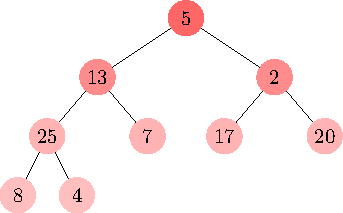
\includegraphics[scale=0.8]{img/6_4-1/6_4-1_1}
          \caption{}\label{fig:6_4-1_1}
        \end{subfigure}
        \begin{subfigure}[t]{.30\textwidth}
          \centering
          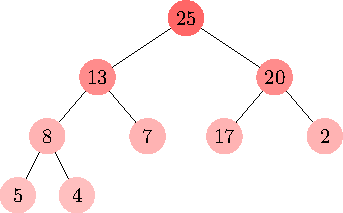
\includegraphics[scale=0.8]{img/6_4-1/6_4-1_2}
          \caption{}\label{fig:6_4-1_2}
        \end{subfigure}
        \begin{subfigure}[t]{.30\textwidth}
          \centering
          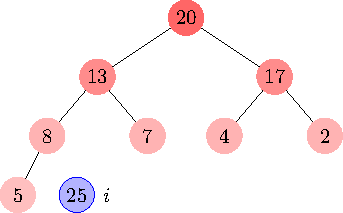
\includegraphics[scale=0.8]{img/6_4-1/6_4-1_3}
          \caption{}\label{fig:6_4-1_3}
        \end{subfigure}
        \begin{subfigure}[t]{.30\textwidth}
          \centering
          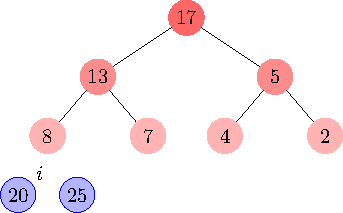
\includegraphics[scale=0.8]{img/6_4-1/6_4-1_4}
          \caption{}\label{fig:6_4-1_4}
        \end{subfigure}
        \begin{subfigure}[t]{.30\textwidth}
          \centering
          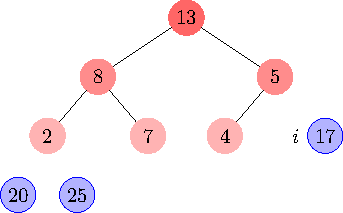
\includegraphics[scale=0.8]{img/6_4-1/6_4-1_5}
          \caption{}\label{fig:6_4-1_5}
        \end{subfigure}
        \begin{subfigure}[t]{.30\textwidth}
          \centering
          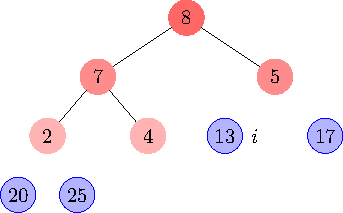
\includegraphics[scale=0.8]{img/6_4-1/6_4-1_6}
          \caption{}\label{fig:6_4-1_6}
        \end{subfigure}
        \begin{subfigure}[t]{.30\textwidth}
          \centering
          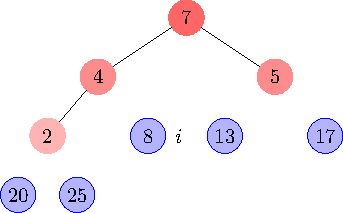
\includegraphics[scale=0.8]{img/6_4-1/6_4-1_7}
          \caption{}\label{fig:6_4-1_7}
        \end{subfigure}
        \begin{subfigure}[t]{.30\textwidth}
          \centering
          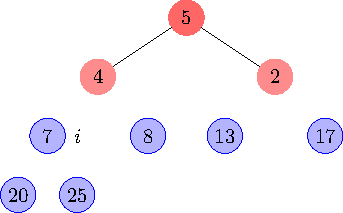
\includegraphics[scale=0.8]{img/6_4-1/6_4-1_8}
          \caption{}\label{fig:6_4-1_8}
        \end{subfigure}
        \begin{subfigure}[t]{.30\textwidth}
          \centering
          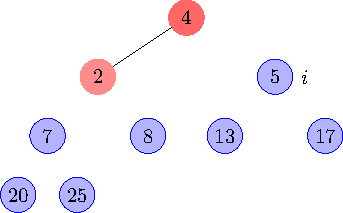
\includegraphics[scale=0.8]{img/6_4-1/6_4-1_9}
          \caption{}\label{fig:6_4-1_9}
        \end{subfigure}
        \begin{subfigure}[t]{.30\textwidth}
          \centering
          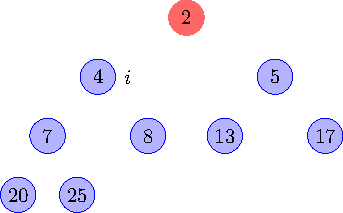
\includegraphics[scale=0.8]{img/6_4-1/6_4-1_10}
          \caption{}\label{fig:6_4-1_10}
        \end{subfigure}
        \caption{Le fonctionnement du $\proc{Heap-Sort}(A)$ sur $A = \langle 5, 13, 2, 25, 7, 17, 20, 8, 4 \rangle$.} 
        \label{fig:Heap-Sort}
      \end{figure}
    \end{ex}
\descitem{6.4-2} \textit{}
    \begin{exrev}
      
    \end{exrev}
\descitem{6.4-3} \textit{}
    \begin{exrev}
      
    \end{exrev}
\descitem{6.4-4} \textit{}
    \begin{exrev}
      
    \end{exrev}
  \item[6.4-5 $\star$]  \textit{}
    \begin{exrev}
      
    \end{exrev}
\end{description}
